\documentclass[a4paper]{article}
\usepackage[top=.75in, bottom=1in, left=1in, right=1in]{geometry}
\usepackage{amsmath}
\usepackage{amssymb}
\usepackage{Sweave}

\title{\vspace{-30pt}STAT 745 -- Fall 2014\\Assignment 4 -- Individual Part}
\author{Doug Raffle}
\date{September 22, 2014}

\renewcommand{\thesubsection}{\thesection.\alph{subsection}}
\setcounter{section}{1}
\DeclareMathOperator*{\argmin}{arg\,min}

\begin{document}
\setlength{\parindent}{0pt}
\vspace{-50pt}
\maketitle

\section{Variable Selection with The LASSO}
\vspace{-30pt}
%Generate Variables:\\
\begin{minipage}[t]{0.45\linewidth}
\end{minipage}

\subsection{$q=0$}
\vspace{-20pt}

\begin{minipage}[c]{0.6\linewidth}
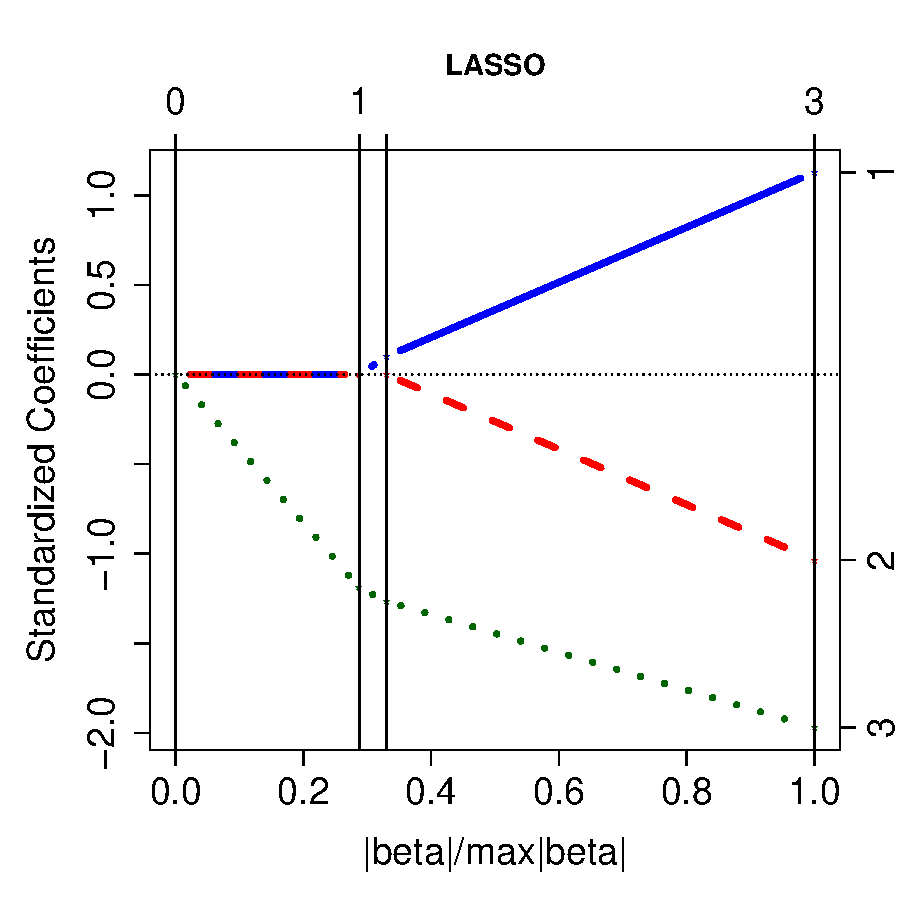
\includegraphics{h4_ind-003}
\end{minipage}
\hspace{-50pt}
\begin{minipage}[c]{0.6\linewidth}
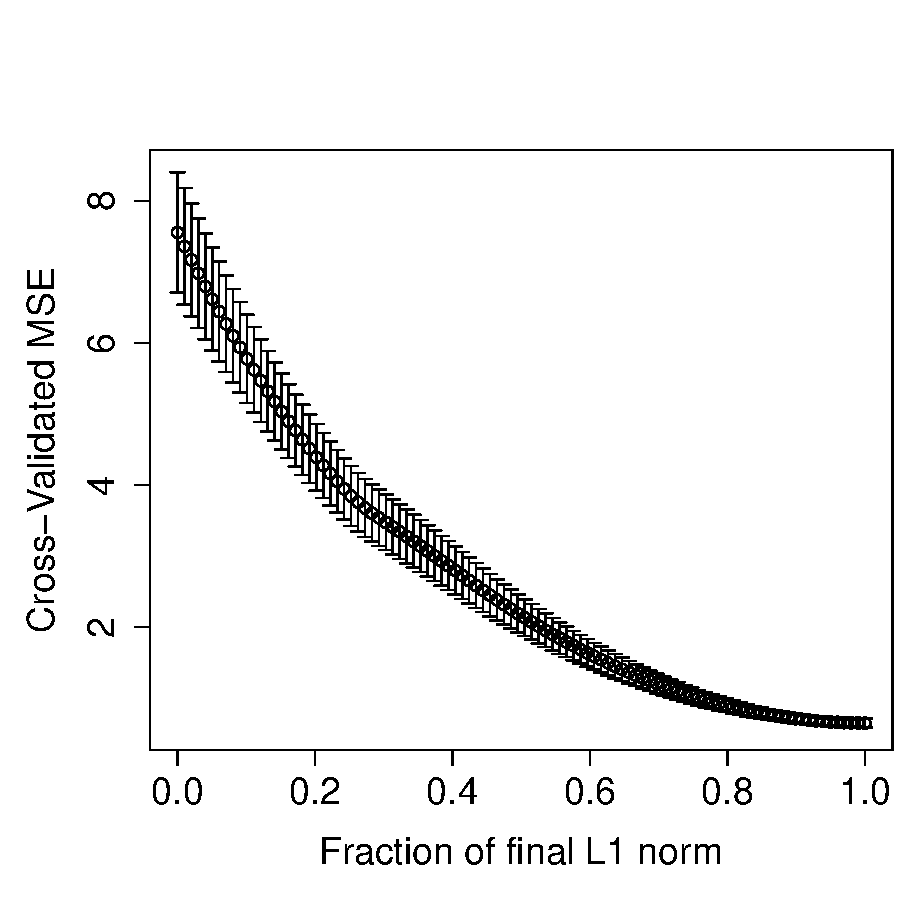
\includegraphics{h4_ind-004}
\end{minipage}

The LASSO is completed in three steps and keeps all three variables in the active set.
$\hat{\beta}_3$, which is has the largest magnitude, is selected first.  $\hat{\beta}_1$ and
$\hat{\beta}_2$ are selected in the second and third step, which makes sense as they differ
in sign, but not magnitude.  As the number of iterations increases, the estimates
get closer to the known values.\\

The model has the lowest MSE when $||\beta||^1_1/\max ||\beta||^1_1=1$,
which is when we have all of the $x_i$'s are included in the model.

\subsection{$\mathbf{q=10}$}
\vspace{-15pt}
\begin{minipage}[c]{0.6\linewidth}
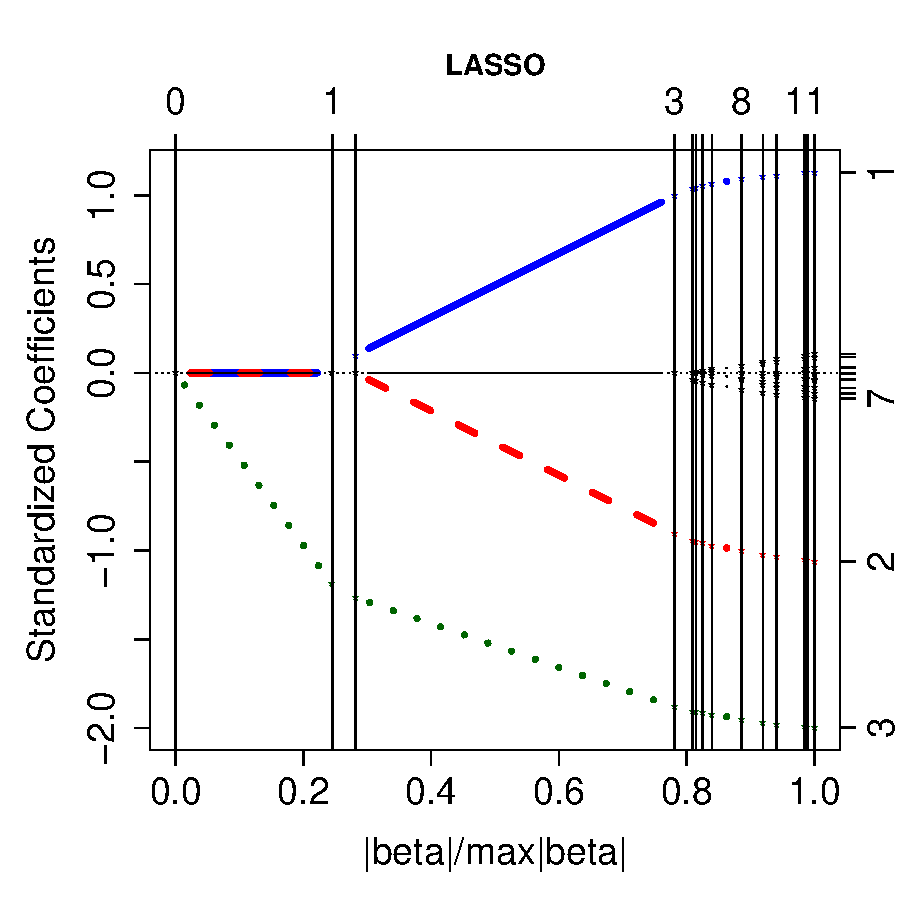
\includegraphics{h4_ind-005}
\end{minipage}
\hspace{-50pt}
\begin{minipage}[c]{0.6\linewidth}
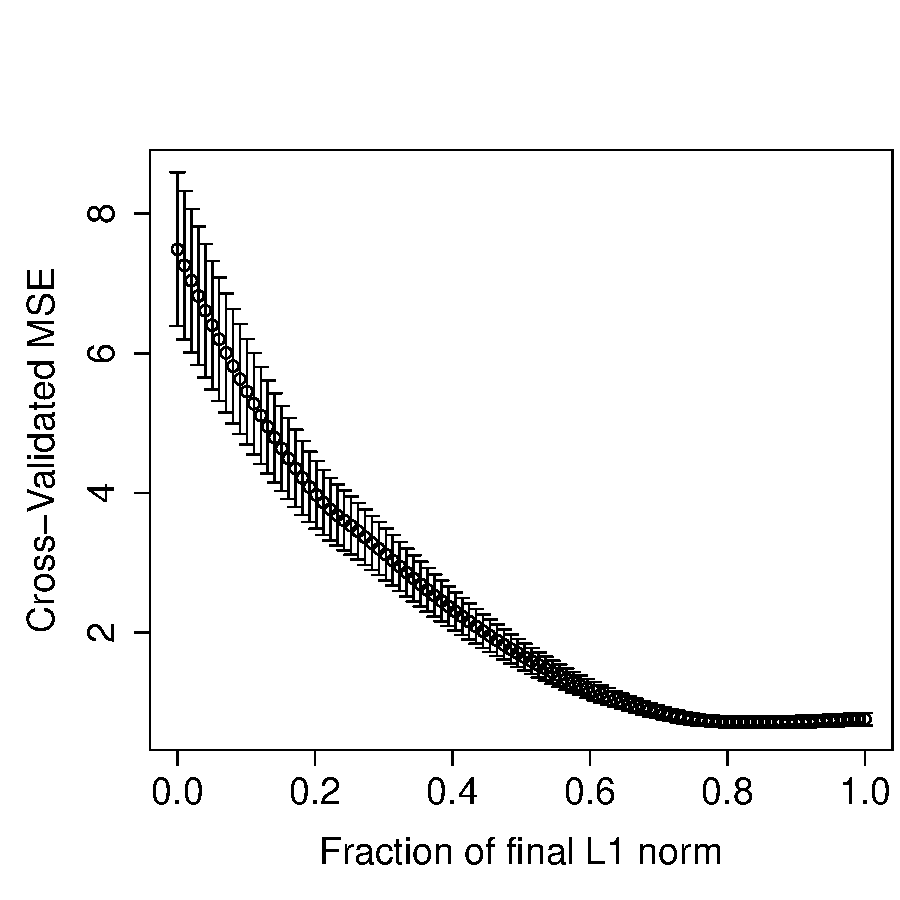
\includegraphics{h4_ind-006}
\end{minipage}\\
The L1 norm ratio levels out right around $0.8$, which is where
the LASSO selected the original three $X$ variables.  The estimates
are not quite at their true values at this point, but they are fairly
close and only marginally improved by increasing the active set.\\

\subsection{$\mathbf{q=50}$}
\vspace{-15pt}
\begin{minipage}[c]{0.6\linewidth}
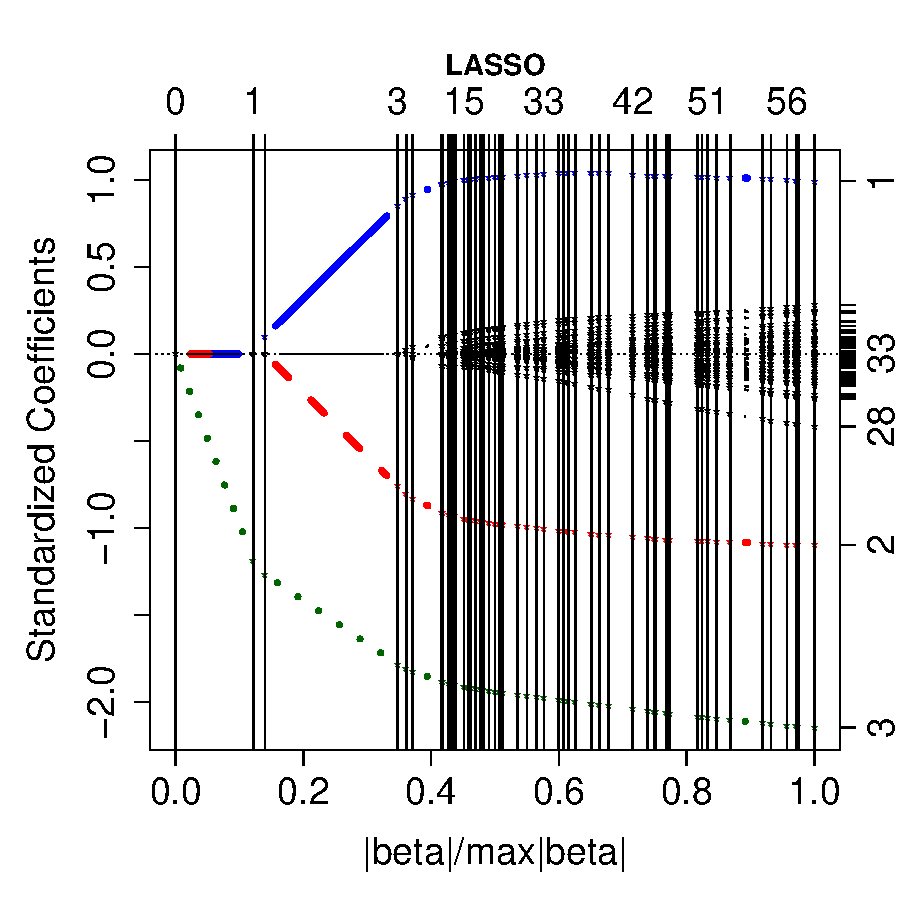
\includegraphics{h4_ind-007}
\end{minipage}
\hspace{-50pt}
\begin{minipage}[c]{0.6\linewidth}
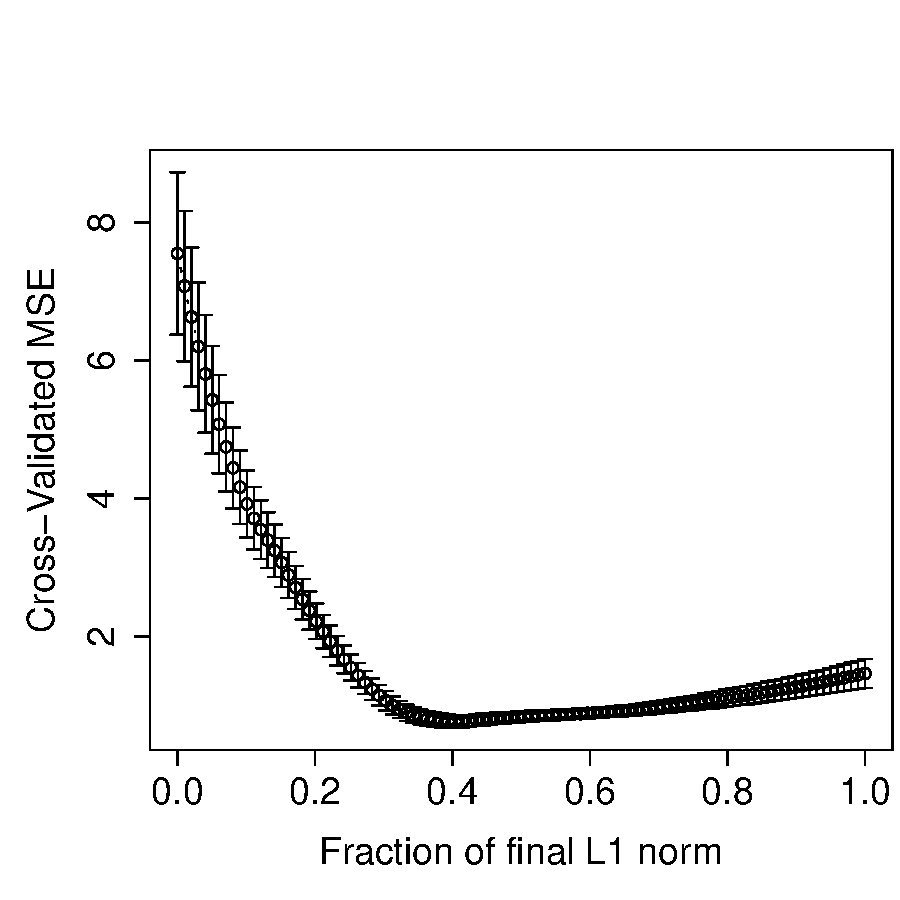
\includegraphics{h4_ind-008}
\end{minipage}
Again, the $X$ variables come in the same way they did when $q=0$:
$x_3$ followed by $x_1$ and $x_2$.  The MSE decreases
quickly as the $x_i$'s are added, and starts to move upward
as the $z_i$'s are included and there is more noise in the data.\\

The problems that occured in $q=10$ are expounded, as the coefficient estimates
are further from their true values when the MSE is optimal.  Additionally, the
estimates are further away from their true value when the full subset is
included (i.e., the magnitude of $\hat{\beta}_3$ is overestimated and $\hat{\beta}_1$
is underestimated).

\subsection{$\mathbf{q=75}$}
\vspace{-15pt}
\begin{minipage}[c]{0.6\linewidth}
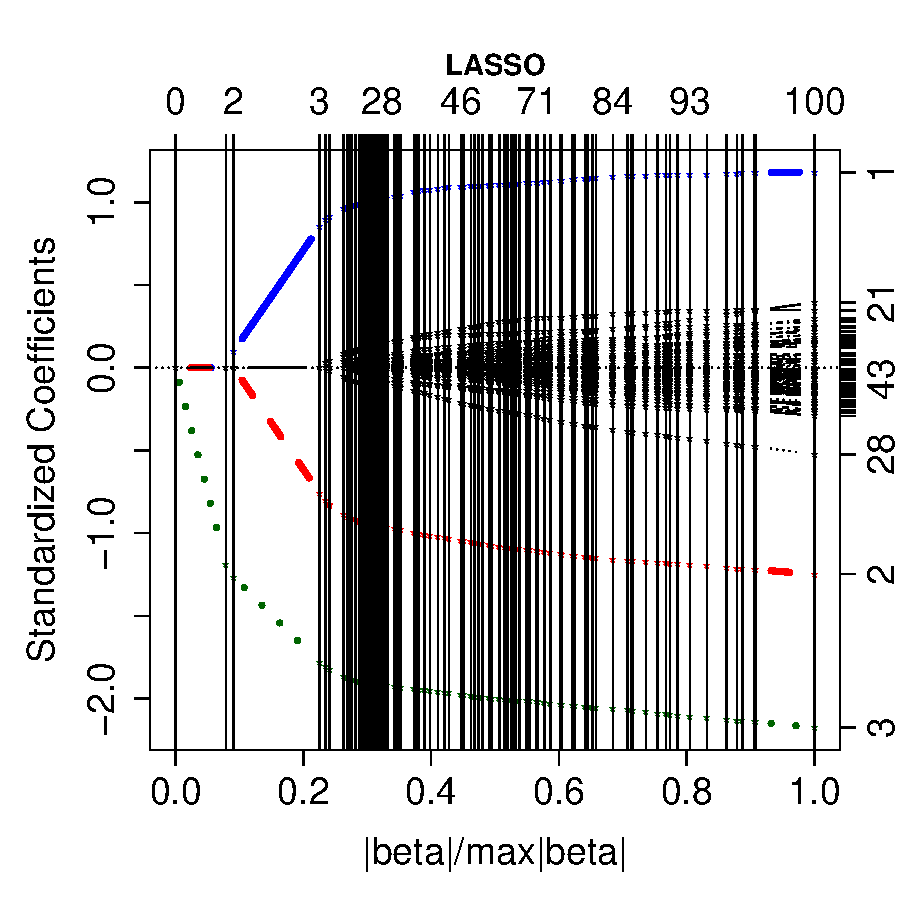
\includegraphics{h4_ind-009}
\end{minipage}
\hspace{-50pt}
\begin{minipage}[c]{0.6\linewidth}
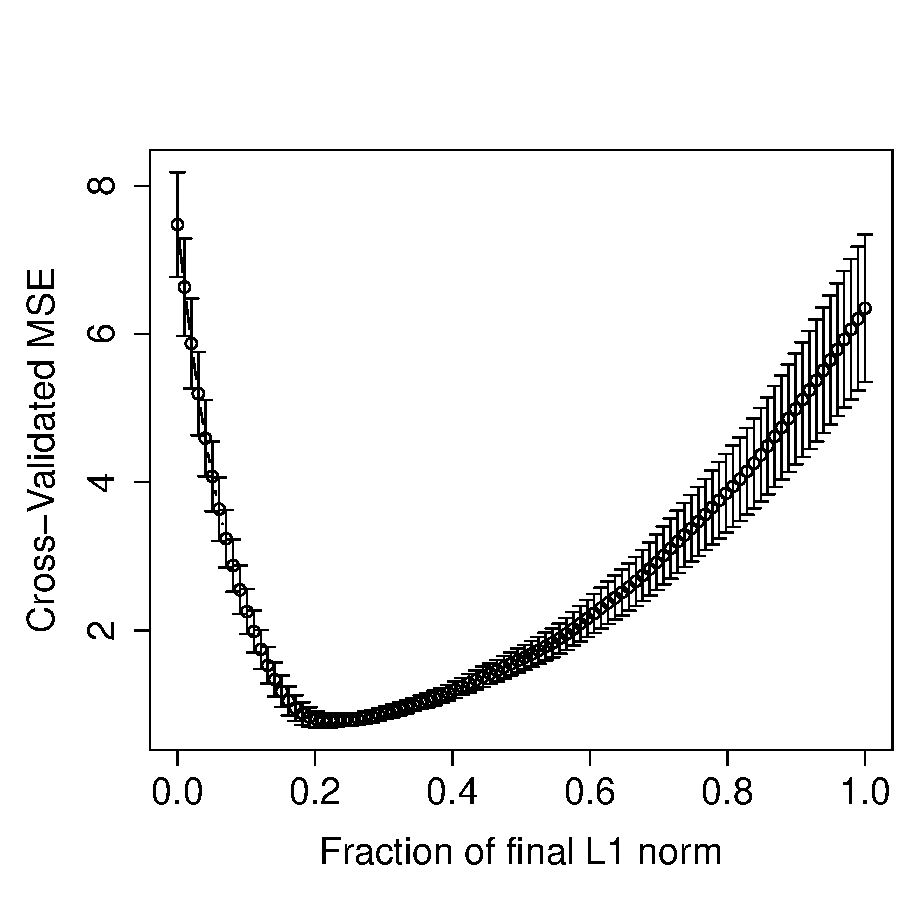
\includegraphics{h4_ind-010}
\end{minipage}\\
The MSE is still minimized when all of the $x_i$'s are included without any
$z_i$'s, and gets worse as more nuisance variables are included.\\

The coefficient estimates are further off both at the optimal MSE and
when the full subset is included than they were when $q=50$.\\

These behaviors are a general trend, and can be seen as $q$ continues
to increase:\\

\subsection{$\mathbf{q=90}$}
\vspace{-15pt}
\begin{minipage}[c]{0.6\linewidth}
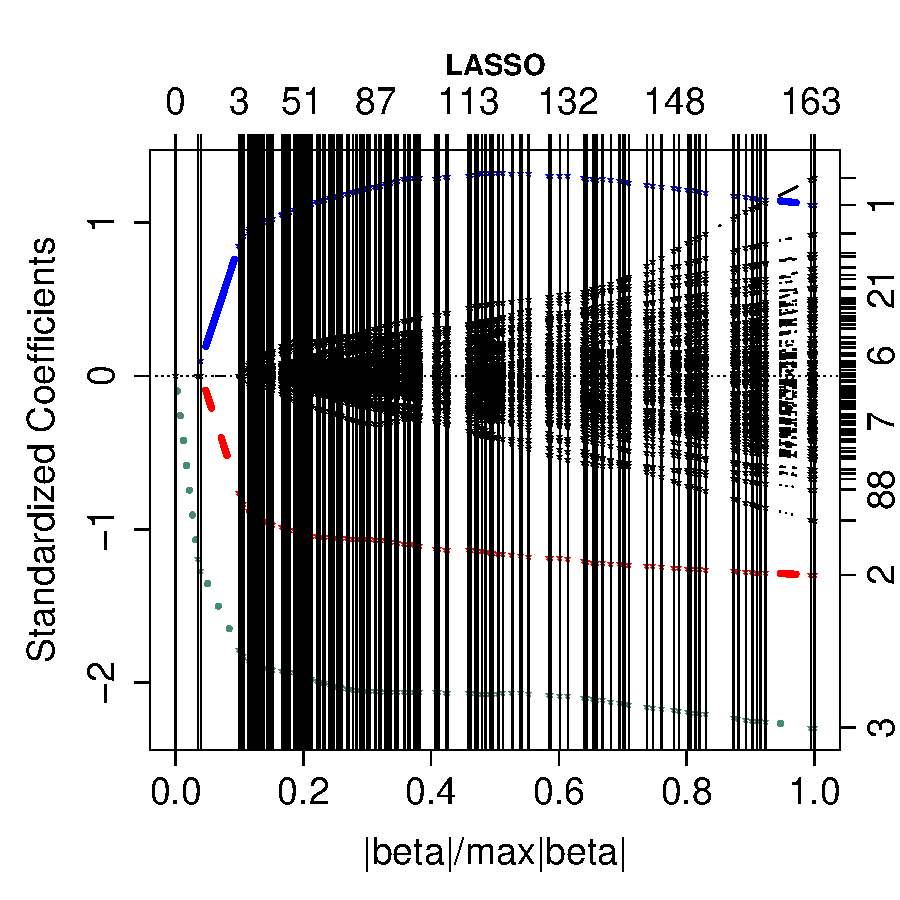
\includegraphics{h4_ind-011}
\end{minipage}
\hspace{-50pt}
\begin{minipage}[c]{0.6\linewidth}
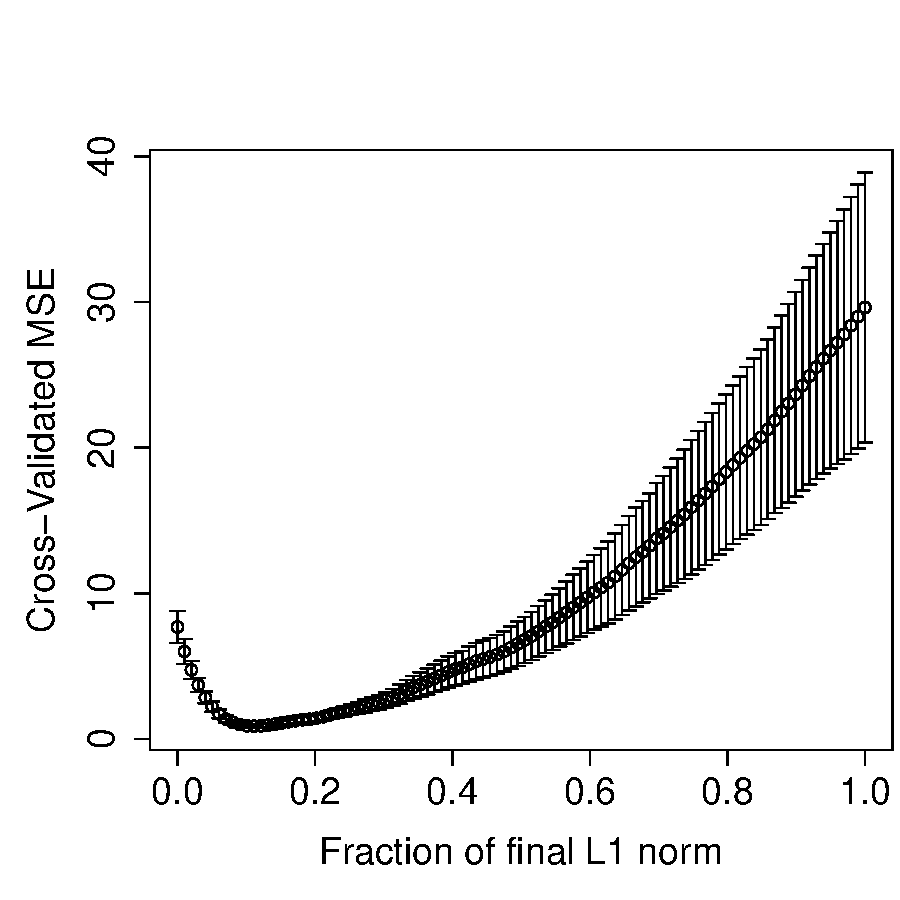
\includegraphics{h4_ind-012}
\end{minipage}

\subsection{$\mathbf{q=99}$}
\vspace{-15pt}
\begin{minipage}[c]{0.6\linewidth}
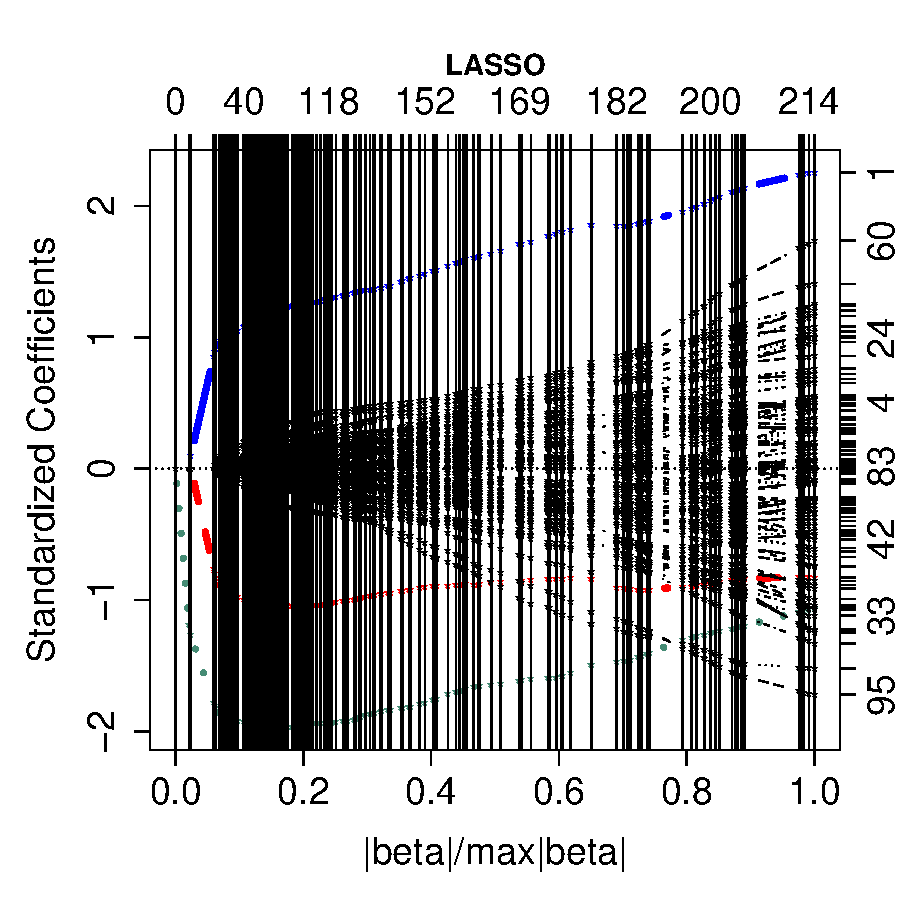
\includegraphics{h4_ind-013}
\end{minipage}
\hspace{-50pt}
\begin{minipage}[c]{0.6\linewidth}
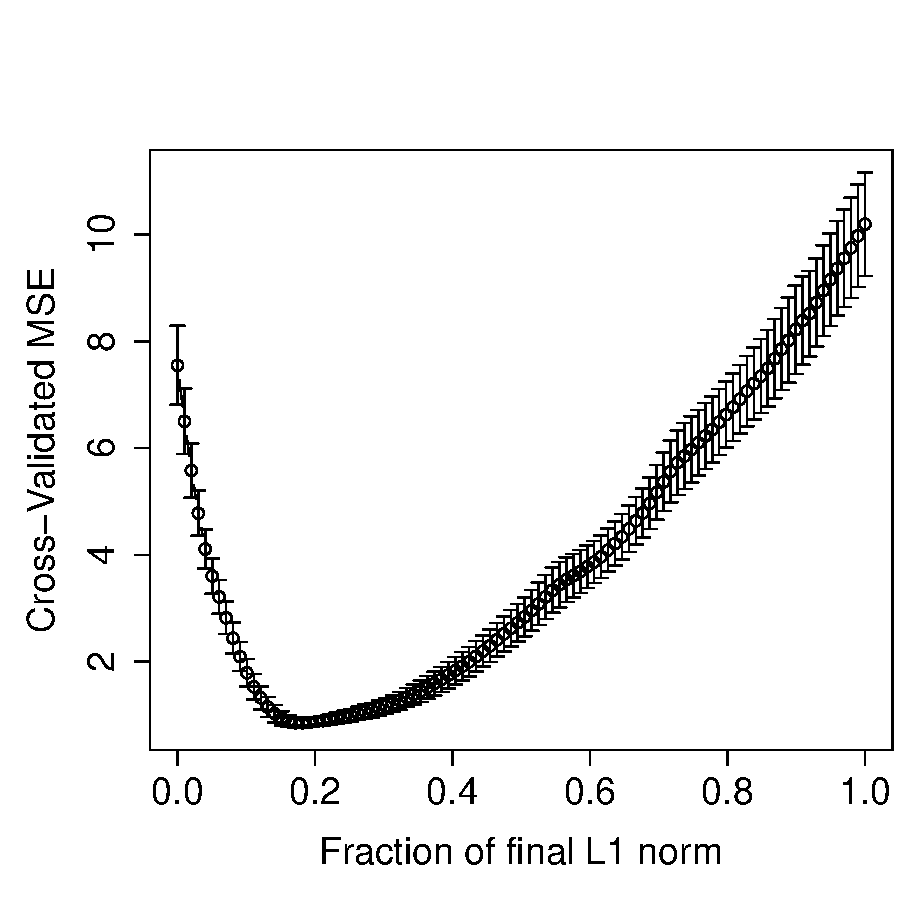
\includegraphics{h4_ind-014}
\end{minipage}\\

It is clear that when the MSE is optimal, all of the $x_i$'s are included
without any $z_i$'s.  Increasing the number of uninformative variables
decreases the precision of the coefficient estimates at this point.\\

The models are increasingly unstable, and the coefficient estimates for the
full subset increasingly worse, as more nuisance variables
are considered.  This is most apparent when $q=99$, where $\hat{\beta}_2$
and $\hat{\beta}_3$ seem to be moving back towards zero, while $\hat{\beta}_1$
continues to increase well past its true value.  More weight continues to
be given to the nuisance variables' coefficients in the full set as $q$ increases, as well.\\

\end{document}
